\label{chap2}

This chapter describes the dynamic model derivation of the soft robotic manipulator. First, the soft robotic system used in this work is further detailed. Then the configuration space of the soft robot is described. Once this configuration space is determine the forward kinematics at position and velocity level are derived. These forward kinematics allow to derive a dynamic model. 


%%%%%%%%%%%%%%%%%%%%%%%%%%%%
%%%%%%%%%%%%%%%%%%%%%%%%%%%%

The soft actuator studied in this work is made from an elastic polymer using selective laser sintering technology. It consists of two bellows placed in parallel. The outside of the bellows are connected, forming the centre line of the actuator. Furthermore, the bellows are connected by a flange at the top and bottom. The soft robot can be pneumatically actuated using air pumps. Each bellow can be inflated individually via a air inlet at one end of the actuator. This flange will be fixed to the ground. The other end is closed, allowing to pressurize the bellows. The actuators geometry and material choice allows the bellows to extend when pressurized. Since each bellow can be inflated independently, the entire actuator can increase its length and change orientation. The actuator is actuated in a single plane, hence the name planar soft robot. 

A kinematic description of the actuator is necessary to describe the position in three-dimensional space. A widely adopted method for describing the configuration of soft robots is piece-wise constant curvature (PCC) modelling \cite{ccapproach}. Previous research used this model to describe forward kinematics of soft actuators are \cite{mahl2014bhakin}, \cite{berkers},\cite{Falkenhahn2015}, \cite{ccapproach}, \cite{runge2017framework}. A schematic drawing of the constant curvature modelling approach is shown in Figure \ref{fig2:ccapproach}. Although we will not be using this exact methodology, it is important to understand the basics. The constant curvature describes the position of the actuator by three coordinates. Parameter $l$ is the curved length of the actuator measured from the fixed bottom to the tip. Coordinate $\kappa$ expresses the curvature of the actuator. It is assumed that the deformed actuator describes a perfect arc, hence radius $r$ is equal to $\frac{l}{k}$. This allows to write the orientation of the actuator's tip as $\theta = l\kappa$. Lastly, parameter $\phi$ describes the rotation of the actuator with respect to the ground. A single constant curvature is not able to describe complex actuator configurations. To this end, multiple of these curves are stacked onto each other, thereby discretizing the actuator. This allows to describe more complex configurations. This methodology is used in for instance \cite{Falkenhahn2015}.

The PCC approach has some limitations, due to its piece-wise character the actuator configuration is not described by a single continuous function. This makes it harder to find analytical expressions for for instance derivatives. Additionally, this PCC approach only allows to assign material properties to particular points. This makes dynamical models generally less accurate. One method to overcome this problem is using partial differential equations (PDE's) to describe actuator configurations. These PDE's are more suitable for deriving continuum dynamic models. 




\begin{figure}[H]
  \begin{minipage}{\linewidth}
      \centering
      \begin{minipage}{0.45\linewidth}
        \begin{figure}[H]
        \centering
        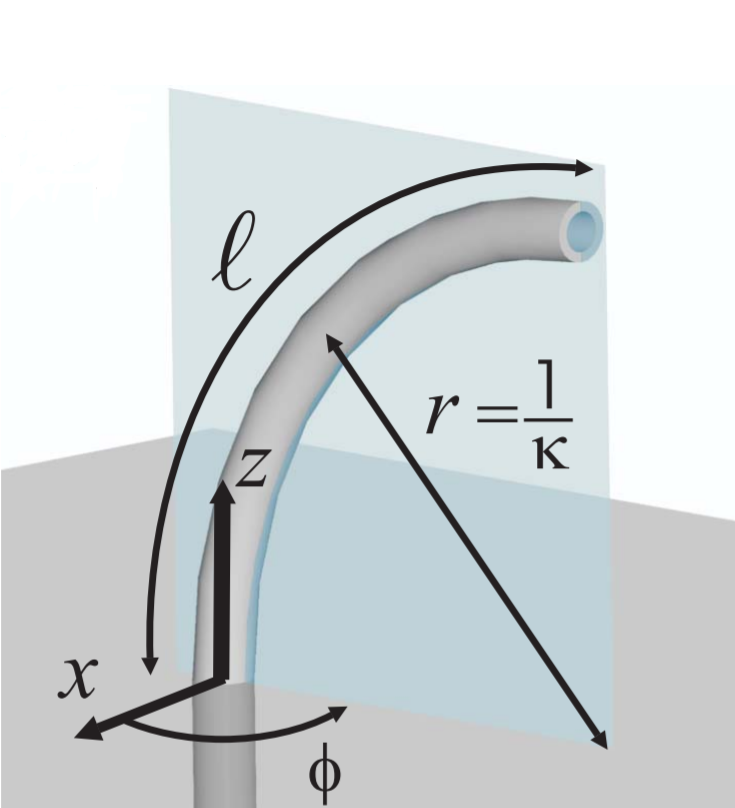
\includegraphics[width=0.85\linewidth]{Figures/Chapter2/ccapproach.png}
         \caption{Schematic drawing of the constant curvature \cite{ccapproach}.}
         \label{fig2:ccapproach}
        \end{figure}
      \end{minipage}
      \hspace{0.05\linewidth}
      \begin{minipage}{0.45\linewidth}
          \begin{figure}[H]
                 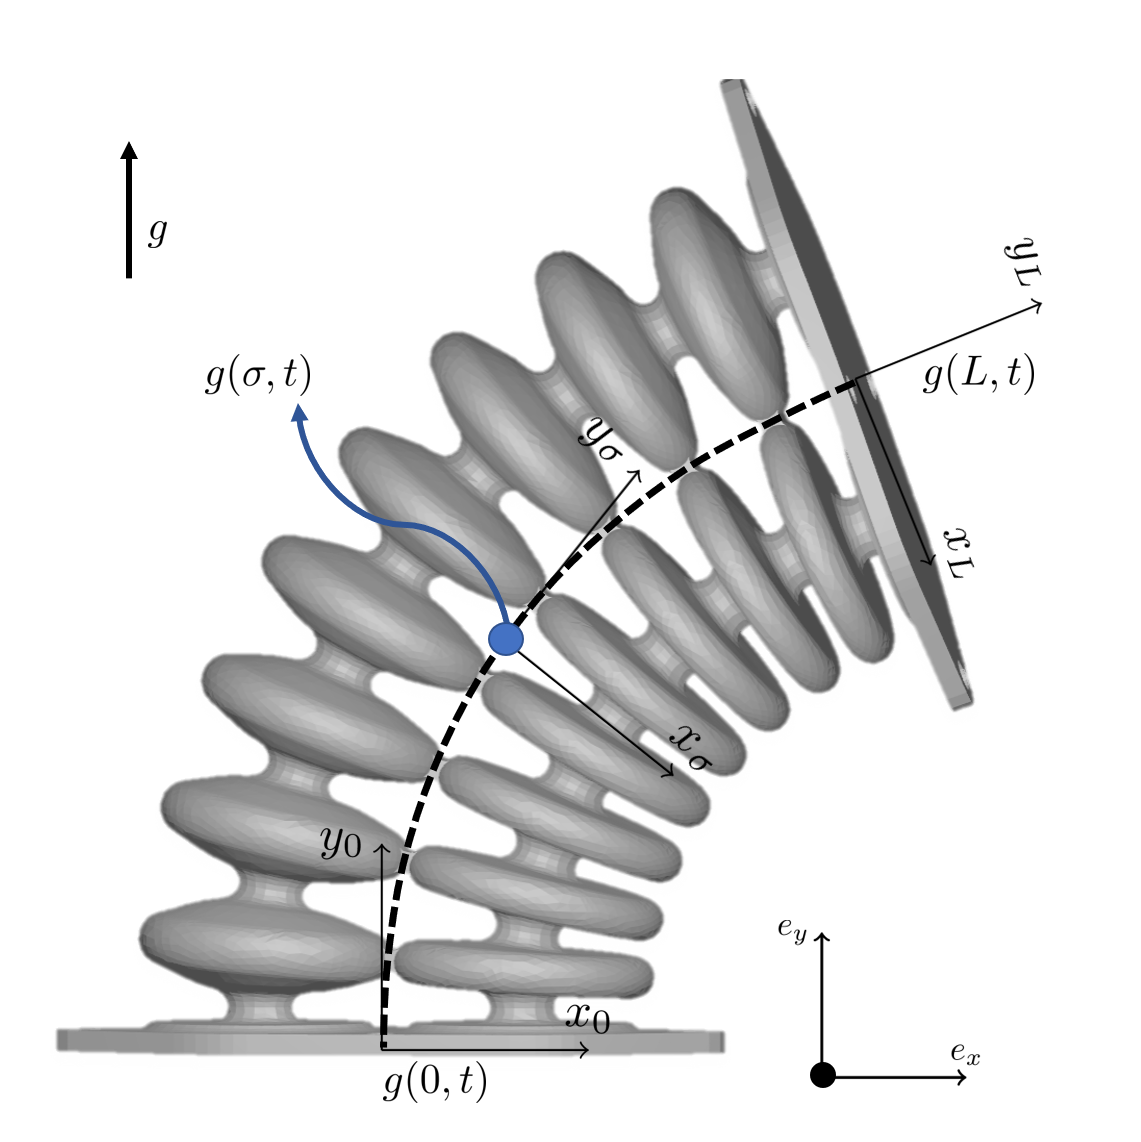
\includegraphics[width=0.88\textwidth]{Figures/Chapter2/actuatorschematic.png}
            \caption{Planar soft actuator with the backbone curve $g(\sigma,t)$.}
            \label{fig2:kinematicschematic}
          \end{figure}
      \end{minipage}
  \end{minipage}
\end{figure}




\section{Configuration space of the soft robot}

To describe the kinematics of the soft actuator used in this study, a Cosserat beam model is used \cite{Boyer2019}. This beam model can be thought of as a continuous one-dimensional curve representing the robot's backbone. This backbone is represented in Figure (\ref{fig2:kinematicschematic}) as the black dashed curve. This curve describes the configuration of the soft robot as a function of space and time. To this end, a spatial coordinate  $\sigma \in \mathbb{X}$ within bounded domain $\mathbb{X} \in [0,l] \subset \mathbb{R}$ is introduced. Furthermore, a temporal coordinate $t \in  \mathbb{T}$ with $\mathbb{T} \subseteq \mathbb{R}$ is defined. This allows to describe position $p(\sigma,t) \in \mathbb{R}^3$ and rotation $R(\sigma,t) \in \mathbb{SO}(3)$ for any point $\sigma$ and time instance $t$ among the backbone of the soft manipulator by \cite{Caasenbrood2020},


\begin{equation}
    g(\sigma,t) = \begin{pmatrix}  R(\sigma,t) & p(\sigma,t) \\ 0_3^\top & 1 \end{pmatrix} \in \mathbb{SE}(3),
    \label{eq2:g}
\end{equation}

where $\mathbb{SE}(3)$ is the Lie group of rigid body transformations in $\mathbb{R}^3$ \cite{Sola2018}. Essentially, function $g(\sigma,t)$ expresses stretch-strain in a local frame evaluated at instance $\sigma$ at time $t$. Before the forward kinematics are derived the following assumption is made.

\begin{manualtheorem}{2.1}[]
Curve  $g(\sigma,t)$ is a continuous differential function $ \forall t \in 
\mathbb{T} $ and $\forall \sigma \in \mathbb{X}$
\end{manualtheorem}

The forward kinematic problem can be found by differentiating (\ref{eq2:g}) with respect to position.
Derivatives with respect to the spatial domain will be indicated with a `prime'. This results in the following partial differential equation (PDE), 




\begin{equation}
   g' = \frac{\partial g}{\partial \sigma} = g \hat{\xi} \hspace{10pt} \text{with} \hspace{10pt}  \hat{\xi} = \begin{pmatrix} K_\times & E \\ 0_3^\top & 0 \end{pmatrix} \in  \mathfrak{se}(3)
    \label{eq2:dgdsigma}
\end{equation}

where $\hat{\xi}$ is the space-twist field. Here, $K_\times \in \mathbb{R}^{3\times 3}$ is a skew-symmetric matrix expressing curvature-torsion strain, and $E = [\epsilon_1,\epsilon_2,\epsilon_3]^\top \in \mathbb{R}^3$ containing stretch-shear strain. The entries of $E$ represent degrees-of-freedom that allow elongation in all three directions. Likewise, the skew-symmetric matrix $K_{\times}$ holds three rotational degrees of freedom. From this skew symmetric matrix vector $K \in \mathbb{R}^3$ can be found. To find $K$ it must hold that $K_\times V = K \times V$ for any $V \in \mathbb{R}^3$ \cite{Boyer2019}. This gives $K = [\kappa_1,\kappa_2,\kappa_3]^\top$ expressing curvatures in all three directions. The stretch-strain and curvature-torsion components will be stored in vector $\xi \in \mathbb{R}^6$ as $[K \hspace{5pt} E]^\top$.

Similar to the spatial derivative, backbone curve $g(\sigma,t)$ can be differentiated with respect to time. These time derivatives will be indicated with a `dot'. This differentiation results in, 

\begin{equation}
  \Dot{g} = \frac{\partial g}{\partial t} = g \hat{\eta} \hspace{10pt} \text{with} \hspace{10pt}  \hat{\eta} = \begin{pmatrix} \Omega_\times & V \\ 0_3^\top & 0 \end{pmatrix} \in  \mathfrak{se}(3)
    \label{eq2:dgdt}
\end{equation}

which describes the time-twist field in a local frame at $\sigma$. Here, $\Omega_\times \in \mathbb{R}^{3 \times 3}$ is a skew-symmetric matrix expressing angular velocity, and vector $V = (v_1,v_2,v_3)^\top \in \mathbb{R}^3$ contains linear velocities. Therefore, $\eta$ effectively describes velocities among the backbone curve. Again, the skew-symmetric matrix $\Omega_\times$ can be represented as a vector $\Omega = [\omega_1,\omega_2,\omega_3]^\top \in \mathbb{R}^3$. These velocities are stored in vector $\eta(\sigma,t) = [\Omega \hspace{5pt} V]^\top \in \mathbb{R}^6$.

\section{Forward velocity kinematics}



Using the equality of mixed partial derivatives, at each instant of space and time $\frac{\partial}{\partial t}g' = \frac{\partial}{\partial \sigma}\dot{g}$ holds \cite{Caasenbrood2020}. Substituting (\ref{eq2:dgdsigma}) and (\ref{eq2:dgdt}) into this relation and simplifying results in,

\begin{equation}
    \hat{\eta}' = -(\hat{\xi}\hat{\eta} - \hat{\eta}\hat{\xi}) + \Dot{\xi},
        \label{eq2:pde2}
\end{equation}

here the Lie bracket $\xi$ and $\eta$ can be recognized between the parenthesis. The Lie bracket $[\hat{\xi},\hat{\eta}]$ also belongs to the group of Lie algebra $\mathfrak{se}(3)$. Therefore, it can be expressed by the adjoint action between $\xi$ onto $\eta$. This adjoint action maps the PDE of (\ref{eq2:pde2}) from $\mathbb{R}^{6\times 6}$ to $\mathbb{R}^6$. This allows to write the velocity kinematics in vector notation as,

\begin{equation}
    \eta'= -\text{ad}_\xi \eta + \Dot{\xi} \hspace{10pt} \text{with} \hspace{10pt} \text{ad}_{\xi} = \begin{bmatrix} K_\times & 0_{3\times 3} \\ E_\times & K_\times \end{bmatrix}.
    \label{eq2:etapde}
\end{equation}


Exploiting the relation $\frac{d}{d \sigma} \text{Ad}_g = \text{Ad}_g \text{ad}_{g^{-1}g'}$ \cite{Boyer2019}, \cite{traversaro2016multibody} , with $g^{-1}g' = \xi$ which follows from (\ref{eq2:dgdsigma}), it follows that $-\text{ad}_\xi = (\text{Ad}_g^{-1})'\text{Ad}_g$. Substitution of this expression into (\ref{eq2:etapde}) allows to formulate the spatial derivative of the velocity twist as,

\begin{equation}
    \eta'= (\text{Ad}_g^{-1})'\text{Ad}_g \eta + \Dot{\xi} \hspace{10pt} \text{with} \hspace{10pt} \text{Ad}_g = \begin{bmatrix} R & 0_{3\times 3} \\ p_\times R & R \end{bmatrix}
    \label{eq2:etadif}
\end{equation}

where $\text{Ad}_g \in \mathbb{R}^{6 \times 6}$ and $\text{Ad}_{g^{-1}}  \in \mathbb{R}^{6 \times 6}$ are the adjoint and inverse adjoint mapping of $g$, respectively \cite{Sola2018}. An analytic solution can be found by integrating (\ref{eq2:etadif}) over spatial domain $[0,\sigma]$. However, solving PDE's is generally more computationally expensive and makes controller design hard.
To overcome this, the theoretical infinite dimensional system is projected onto a finite dimensional subspace. In order to do so, we assume the following.


\begin{theorem}

For any $t \in \mathbb{T}$ and $\sigma \in \mathbb{X}$, strain $\xi(\sigma,t)$ can be written as an infinite expansion of the form \cite{Caasenbrood2021},

\begin{equation}
\xi_i(\sigma,t) = \sum_{i=1}^\infty \varphi_i(\sigma)q_i(t) + \xi_{i,0}(\sigma), \hspace{20pt} \forall \sigma \in \mathbb{X}, t \in \mathbb{T},
\label{eq2:strainexact}
\end{equation}

in which, $\xi_{i,0}$ corresponds to the internal strains of the undeformed configuration of the robotic manipulator, $\{\varphi_i\}_{i \in \mathbb{N}}$ is a set of basis shape functions and $q(t)$ are modal coefficients. 
\end{theorem}

Essentially, the PDE of (\ref{eq2:dgdsigma}), is transformed to an ordinary differential equation (ODE) by exploiting the Galerkin reduction method \cite{Galerkin}.



Here, the infinite dimensional system is projected onto a subspace of finite dimension that contains basis elements of the expected solution. By reducing the dimensionality of the system, higher order dynamics are not captured in the model and thus robustness should be taken into account. To transform PDE (\ref{eq2:dgdsigma}), the components of the strain field $\xi(\sigma,t)$ are approximated using a finite amount of shape functions as,

\begin{equation}
    [\xi_i(\sigma,t)]_N = \sum_{i=1}^N \varphi_i(\sigma)q_i(t) + \xi_{i,0}(\sigma), \hspace{20pt} \forall \sigma \in \mathbb{X}, t \in \mathbb{T},
    \label{eq2:strainapprox}
\end{equation}

where $N$ is the amount of shape functions used to approximate strain $\xi(\sigma,t)$. It should be clear that the initial internal deformation $\xi_{(i,0)}$ is time invariant. There exist multiple variants of shape function polynomials that can be used in approximating strain. The Chebyshev polynomial, Polynomial and Legendre polynomials are respectively given by,

\begin{equation}
    \varphi_{k,cheby}(\sigma) = \cos(k \sigma), \hspace{40pt} \varphi_{k,poly} = \sigma^k, \hspace{40pt} \varphi_{k,legend} = \frac{1}{2^k k!} \frac{d^k}{d\sigma^k}(\sigma^2-1)^k.
    \label{eq2:shapefunction}
\end{equation}


Each degree of shape-function gives the model a certain amount of flexibility. Therefore increasing the order of shape-functions allows the model to describe more complex robot configurations. To avoid coupling between shape functions,  it is important that these shape functions are orthogonal. This means that $\int_\mathbb{X} \varphi_i \varphi_j d \sigma = 0$ for any $i \neq j$ and non-zero otherwise. Given this, the $N$-th order strain expansion can be formulated as,



\begin{equation}
\begin{aligned}
    \begin{bmatrix}\xi(\sigma,t)\end{bmatrix}_N = & \hspace{5pt}  (B_a \otimes [ \varphi_0 \dots \varphi_N ])q(t)\\ = &  \underbrace{ \begin{pmatrix}
    \varphi_1(\sigma) & \dots  & \varphi_N(\sigma) & \dots     & 0      & \dots  &  0 \\
    \vdots    & \ddots & \vdots    & \ddots    & \vdots & \ddots & \vdots \\
    0         & \dots  & 0         & \dots     & \varphi_0(\sigma) & \dots & \varphi_N (\sigma)
    \end{pmatrix}}_{\Phi(\sigma)} \begin{pmatrix} q_1(t) \\ \vdots \\ q_n(t) \end{pmatrix} +  \begin{pmatrix} \xi_{1,0} \\ \vdots \\ \xi_{n,0}   \end{pmatrix}
    \end{aligned},
\label{eq2:xishape}
\end{equation}

where $\Phi \in \mathbb{R}^{m \times n}$ is a shape function matrix where $n$ is equal to the amount of modal coordinates, and $m$ the amount of active strains, and $B_a \subseteq \text{span}(\mathbb{I}_6)$ a selection matrix of unconstrained strains. It should be clear that modal coordinate vector $q(t)$ has length $m \times N$.

Now we have an approximation for the strain of the actuator, we can find the analytic solution to the  velocity-twist field (\ref{eq2:etadif}). It is given that the actuator is fixed at one end. Therefore the boundary conditions $\eta_0 = 0_{6 \times 1}$ and $g_0 = I_{4\times 4}$ can be imposed. This physically means that at $\sigma = 0$ there is no velocity, strain nor curvature.  Integrating over domain $[0,\sigma]$ will give accordingly \cite{Caasenbrood2020},

\begin{equation}
  \begin{bmatrix} \eta(\sigma,t)\end{bmatrix}_N = \text{Ad}_{[g]_N^{-1}} \int_0^{\sigma} \text{Ad}_{[g]_N} B_a \Phi(\sigma) d \sigma \dot{q} = J\dot{q}
    \label{eq2:J}
\end{equation}

here an expression for the geometric Jacobian $J(\sigma,t) \in \mathbb{R}^{6\times n}$ is obtained. This Jacobian maps modal coordinate velocity to linear and angular velocities among the backbone curve. This results in a Jacobian matrix which is non-linear with respect to position and time. This Jacobian will of use in determining the system dynamics. Furthermore it can be used for determining inverse kinematics, and control purposes.

%Given (\ref{eq2:J}) and the boundary condition $\dot{\eta}_0 =0_{6\times 1}$, the kinematics at acceleration level can be given as,

%\begin{equation}
%    \dot{\eta}(\sigma,t) = \text{Ad}_g^{-1} \int_0^{\sigma} \text{Ad}_{g} B_a \Phi(\sigma) d \sigma \ddot{q}(t) +  \text{Ad}_g^{-1} \int_0^{\sigma} \text{Ad}_{g} \text{ad}_\eta B_a \Phi(\sigma) d \sigma \ddot{q}(t) = J\ddot{q} + \dot{J}\dot{q},
%\end{equation}

%where a time derivative of the Jacobian can be seen. Both expressions will be of use in determining the dynamics of the system.

We have now presented a general framework for modelling forward kinematics for soft robots. Before deriving the actuator dynamics, the forward kinematics for the planar actuator will be presented.  This allows to solve the forward kinematic problem by solving (\ref{eq2:dgdsigma}) with an approximation of the strain by (\ref{eq2:strainapprox}). To this end we make the following assumption:


\begin{theorem}
The planar soft actuator can be described by 2 active strains, one extension and one curvature. Out of plane curvature is deemed negligible small.
\end{theorem}

For the planar robot, it shall be clear that we can actuate two degrees of freedom. By pressurizing both bellows equally the actuator can elongate. A difference in bellow pressure will induce a curvature. Therefore two active degrees of freedom are included. In the kinematic model strain $\epsilon_3$ and curvature $\kappa_2$ will take value 1. All other degrees-of-freedom will take value 0. Recall $\xi(\sigma,t)$ is $[K \hspace{5pt} E]^\top$, this results in vector $[0,1,0,0,0,1]^\top$. Selection matrix $B_a$ will have the following structure,

\begin{equation}
    B_a = \begin{bmatrix}
    0 & 1 & 0 & 0 & 0 & 0 \\
    0 & 0 & 0 & 0 & 0 & 1 \\
    \end{bmatrix}^\top,
\end{equation}

the actuator has an initial length in the $\epsilon_3$ direction. Therefore $\xi_0 = [0,0,0,0,0,1]^\top$. Throughout this work we will use "elongation" or $\epsilon$ to address strain $\epsilon_3$. Likewise, ``curvature'', ``rotation'' or  $\kappa$ are used interchangeably to refer to curvature $\kappa_2$. Lastly, the amount of shape functions used to approximate strains is set. To this end another assumption is made.

\begin{theorem}
Approximation of the strains in the planar actuator with a single shape function will capture general deformation.  
\end{theorem}

Approximating strains and curvatures with a single shape function will reduce this Cosserat model to the constant curvature model. As can be seen from (\ref{eq2:shapefunction}), all shape functions yield 1 for $k=0$. In this case the modal coordinates $q(t)$ will be equal to $\kappa$ and $\epsilon$, respectively. 
From this point onward, only a single shape function is used to approximate the strains and curvatures of the actuator. The forward kinematic model for the planar soft robot is programmed in \MATLAB \cite{MATLAB2020}. Figure (\ref{fig1:forward_kinematic}) shows the result of the forward kinematic model for a first order approximation of strains. The initial position is obtained for zero curvature and elongation. Here it can be seen that the initial length of the actuator is 64.5 mm. To obtain the deformed modal coordinate $q$ was chosen equal to $[-17,0.1]^\top$. 



\begin{figure}[H]
    \centering
    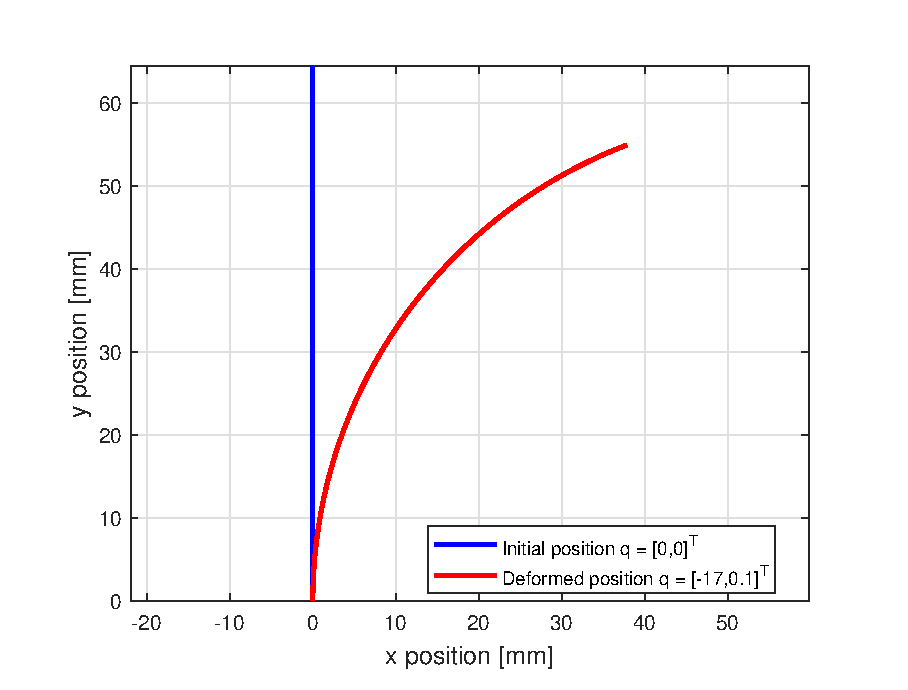
\includegraphics[width = 0.7\textwidth]{Figures/Chapter2/fkin1701.eps}
    \caption{Initial position and deformed position for a first order shape function approximation of the kinematic model.}
    \label{fig1:forward_kinematic}
\end{figure}

Besides a forward kinematic model, a numerical inverse kinematic solver was programmed. This allows to define a position in planar Cartesian coordinates. The algorithm will minimize the distance between the desired end-effector position and reachable end-effector position given an amount of shape functions. It shows the model's flexibility when using multiple shape functions. The algorithm is further detailed in Appendix \ref{app:chap2}. 




%The forward kinematic problem of (\ref{eq2:dgdsigma}) is programmed in \MATLAB \cite{MATLAB2020}. Given modal coordinates $q(t)$ and initial conditions at $\sigma = 0$, the actuator position can be calculated. To reduce computation time, the rotation matrix in (\ref{eq2:g}) is reformulated using quaternion formulation \cite{Boyer2019}. This allows to express any rotation by a vector of length 4, instead of 3 by 3 matrix. Therefore $g(\sigma,t)$ can significantly be reduced from 16 entries, to only 7 entries when using quaternion formulation. Any rotation matrix $R(\sigma,t)$ can be rewritten to quaternions by,


%\begin{equation}
%\frac{\partial g}{\partial \sigma} \equiv \frac{\partial}{\partial \sigma}    \begin{pmatrix} Q \\ p \end{pmatrix} = \begin{pmatrix} 2 ||Q||^{-1} A(R(Q)K)Q \\ R(Q)p \end{pmatrix},
%\label{eq2:Qp}
%\end{equation}

%where $Q \in \mathbb{R}^4$ is the quaternion representation of rotation matrix $R$, and $R(Q)$ a function mapping a quaternion to rotation matrix representation, $A$ is a function defined as,


%\begin{equation}
%    A(K) = \begin{pmatrix} 0 & -K_1 & -K_2 & -K_3 \\ K_1 & 0 & -K_3 & \hspace{8pt}K_2 \\ K_2 & \hspace{8pt}K_3 & 0 & -K_1 \\ K_3 & -K_2 & \hspace{8pt}K_1 & 0 \end{pmatrix},
%    \label{eq2:AK}
%\end{equation}

%where $K_i$ correspond to the entries of $\xi(\sigma,t)$ shown in (\ref{eq2:dgdsigma}). In  (\ref{eq2:Qp}) and (\ref{eq2:AK}) the dependency of $\sigma$ and $t$ has been omitted for the sake of readability.




%%%%%%%%%%%%%%%%%%%%%%%%%%%%%%%%%%%%%%%%%%%%%%%%%%%%%%%%%%%%%%%%%%%%%%%%
%%%%%%%%%%%%%%%%%%%%%%%%%%%%%%%%%%%%%%%%%%%%%%%%%%%%%%%%%%%%%%%%%%%%%%%%
%%%%%%%%%%%%%%%%%%%%%%%%%%%%%%%%%%%%%%%%%%%%%%%%%%%%%%%%%%%%%%%%%%%%%%%%

\section{Dynamic Modelling}


To study the dynamic behaviour of the soft actuator a dynamic model is created. A relatively simple approximation is used to get insight of the basic dynamics of the actuator. In this we propose a non-linear mass-spring-damper model. The developed model incorporates non-linear mass and non-linear stiffness matrix in an effort to increase model accuracy. In this section an analytical expression for the mass matrix is provided. Additionally damping and stiffness matrices are introduced. For which the entries are determined in Chapter \ref{chap3}.

The mass matrix for the dynamical system is derived using a the Euler-Lagrange method \cite{Caasenbrood2020}. Since we have an expression for modal coordinate velocity, the total kinetic energy of the system is given by,


\begin{equation}
    \mathcal{T} = \frac{1}{2}\int_0^{\sigma} \eta(\sigma,t)^\top \mathcal{M} \eta(\sigma,t) d \sigma  = \frac{1}{2}\int_0^{\sigma} (J \dot{q})^\top \mathcal{M} J\dot{q} d \sigma
    \label{eq2:T}
\end{equation}

where $\mathcal{M} \in \mathbb{R}^{6\times6}$ is a diagonal mass matrix. In our modelling approach, the actuator kinematics have been described by a one-dimensional backbone curve. In order to derive the dynamics, mass properties need to be assigned to this curve. Therefore the backbone curve is discretized, and we consider a cross section of the actuator. In determining the mass of the system the following assumption is made. 

\begin{theorem}
Inertial properties of the actuator can be determined by considering an infinitely thin slice in transverse direction, and regarding it as a solid cuboid.
\end{theorem}


Figure (\ref{fig:massapprox}) shows such a discretized cross section. Here the blue marked area is a solid cuboid with height $h$, width $w$, density $\rho$ and slice thickness $d\sigma$. 

\clearpage

\begin{figure}[H]
    \centering
    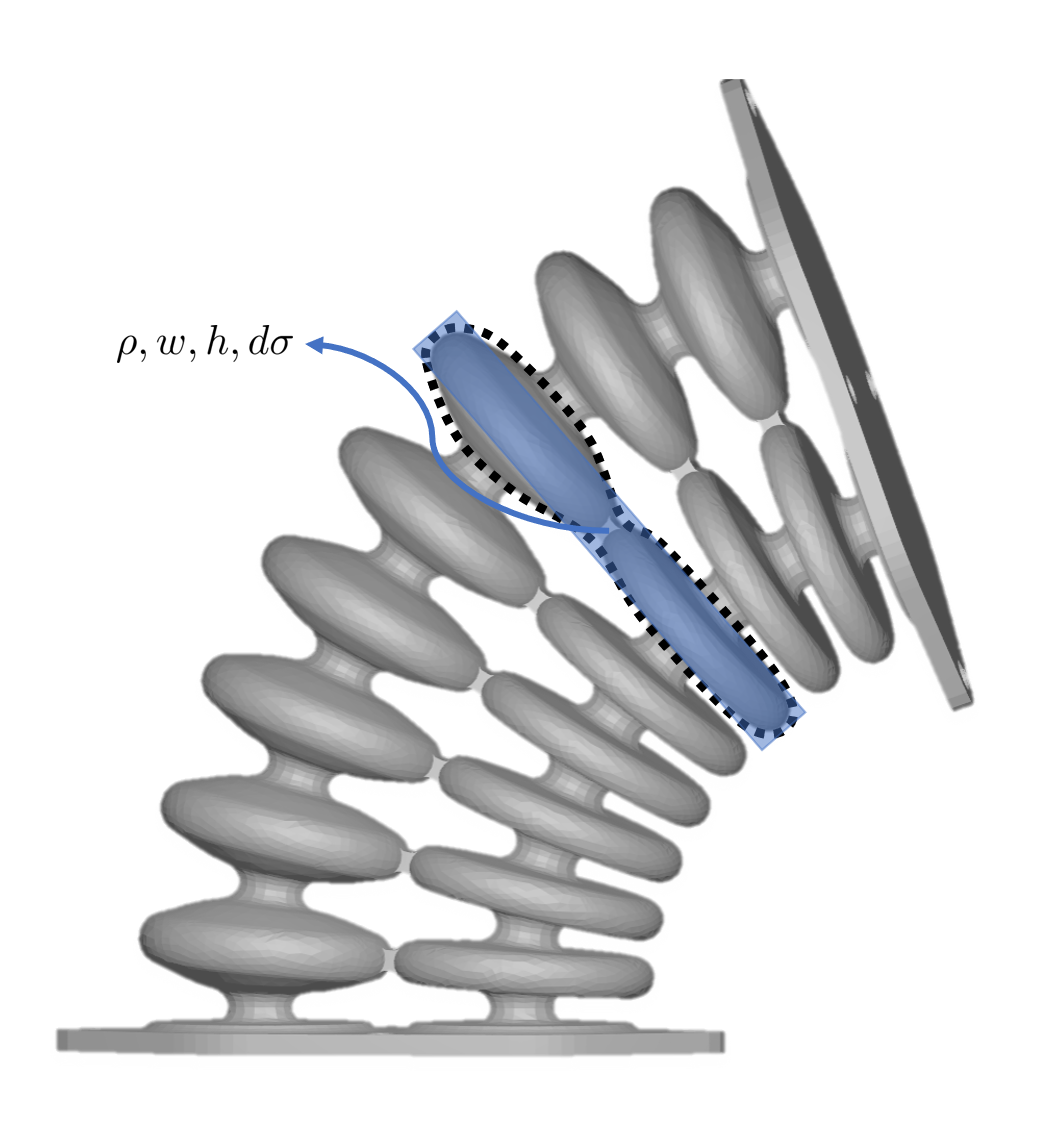
\includegraphics[width = 0.4\textwidth]{Figures/Chapter2/massapprox.png}
    \caption{Inertial properties can be determined by regarding an infinitely thin slice. The cross section is then viewed a solid cuboid.}
    \label{fig:massapprox}
\end{figure}

The mass matrix $\mathcal{M}$ then takes the following form,

\begin{equation}
    \mathcal{M} = \begin{pmatrix} \frac{1}{12}\rho (w^2 + d^2) & 0 & 0 & 0 & 0 & 0 \\
                                  0 & \frac{1}{12}\rho (w^2 + h^2) & 0 & 0 & 0 & 0 \\
                                  0 & 0 & \frac{1}{12}\rho (d^2 + h^2) & 0 & 0 & 0 \\
                                  0 & 0 & 0 & \rho & 0 & 0 \\
                                  0 & 0 & 0 & 0 & \rho & 0 \\
                                  0 & 0 & 0 & 0 & 0 & \rho \end{pmatrix}\hspace{5pt} \text{with} \hspace{5pt} \rho = \frac{m_{tot}}{L_0}
\end{equation} 




where $m_{tot}$ is the total mass of the actuator. The first three entries express mass moments of inertia, related to curvature of the actuator. The last three entries relate to linear velocities of centre of mass of the cuboid. Based on equation (\ref{eq2:T}) the position variant mass matrix can be expressed as, 


\begin{equation}
    M(q) = \int_0^{\sigma} J(\sigma)^\top \mathcal{M}(\sigma)J(\sigma) d \sigma.
\end{equation}

Furthermore damping and stiffness properties are assigned to the actuator. We assume that the polymer of which the actuator is made has linear damping characteristics. An expression for the damping matrix is obtained by,

\begin{equation}
    D = \int_0^\sigma (B_a \Phi(\sigma))^\top  \mathcal{D} (B_a \Phi(\sigma)) d\sigma,
\end{equation}

where $\mathcal{D} \in \mathbb{R}^{6 \times 6}$ is a diagonal damping matrix. For a fact, we know that polymer has non-linear stiffness properties. Therefore stiffness matrix $K$ is position variant, and is therefore given by,

\begin{equation}
    K(q) = \int_0^\sigma (B_a \Phi(\sigma) )^\top \mathcal{K}(q) (B_a \Phi(\sigma))  d\sigma,
\end{equation}

where $\mathcal{K} \in \mathbb{R}^{6 \times 6}$ is a diagonal stiffness matrix. The actuator dynamics that are obtained are then given by,

\begin{equation}
    M(q)\Ddot{q} + D\dot{q} + K(q)q = \tau  \hspace{10pt} \text{with} \hspace{10pt} \tau = Hp,
    \label{eq2:simp_model}
\end{equation}

where $\tau \in \mathbb{R}^2$ describes the input moment and force acting on curvature and elongation, respectively. Since the experimental set-up allows for pressure regulation, a to be determined mapping matrix $H \in \mathbb{R}^{2\times2}$ is introduced. This matrix maps input pressure $p \in \mathbb{R}^2$ to force and torque input vector $\tau$. Due to the low mass of system, Coriolis and gravitational effects have been neglected. Both effects deemed to have a little influence on the system behaviour. In Chapter \ref{chap3} a parameter study is presented. Here we present the methodology to determine elongation and curvature stiffness. Furthermore the force mapping is presented. Both stiffness and input mapping are derived using finite element analysis.



% hspace{10pt} \text{with} \hspace{10pt} u = Hp

%Since the experimental set-up allows for pressure control, a mapping matrix $H \in \mathbb{R}^{2\times2}$ is necessary. This matrix maps input pressure $p \in \mathbb{R}^2$ to force and torque input vector $u \in \mathbb{R}^2$.


%As mentioned, the work of \cite{Caasenbrood2020} describes the %actuator dynamics based on a Lagrangian formulation. This includes the derivation of the Coriolis and gravitational effects. Here the Coriolis effects are described by,

%\begin{equation}
%    C(q,\dot{q}) = \int_0^\sigma J^\top(\mathcal{M})\Dot{J} + J^\top(\mathcal{M}\text{ad}_\eta - \text{ad}_\eta^\top \mathcal{M})J d \sigma,
%\end{equation}

%where $\Dot{J}$ represents the time derivative of the Jacobian matrix. Furthermore, $\text{ad}_\eta$ represents the adjoint action of velocity vector $\eta$. Additionally gravitational effects are captured by,

%\begin{equation}
%    g(q) = \int_0^\sigma J^\top \mathcal{M} \text{Ad}_{g^{-1}} a_z d\sigma
%\end{equation}

%where $a_z \in \mathbb{R}^6$ is a matrix representing the gravitational acceleration. Therefore $a_z = [0,0,0,-9.81,0,0]^\top$.